\documentclass{beamer}

%\usetheme[framenumber,totalframenumber]{UniversiteitGent}
%\usetheme[faculty=di,framenumber,totalframenumber]{UniversiteitGent}
%\usetheme[faculty=we,usecolors,framenumber,totalframenumber]{UniversiteitGent}
%\usetheme[language=english,framenumber,totalframenumber]{AlleghenyCollege}
\usetheme{AnnArbor}
\usecolortheme{dove}

\title{CMPSC 390/Art 387 \\ Crypto Introduction }
\author{Janyl Jumadinova and Byron Rich}
\date{January 19, 2021}

\long\def\omitit#1{}

\usepackage{hyperref}

\begin{document}

\begin{frame}
  \titlepage
\end{frame}

%%%%%%%%%%%% Slide %%%%%%%%%%%%%%%%%%%%%%%%%%%%%%%%%%%%%%%%%%%%%%%%%%%
\begin{frame}
  \frametitle{Cryptocurrency? Crypto? Bitcoin? Blockchain? ... }
  	\centering 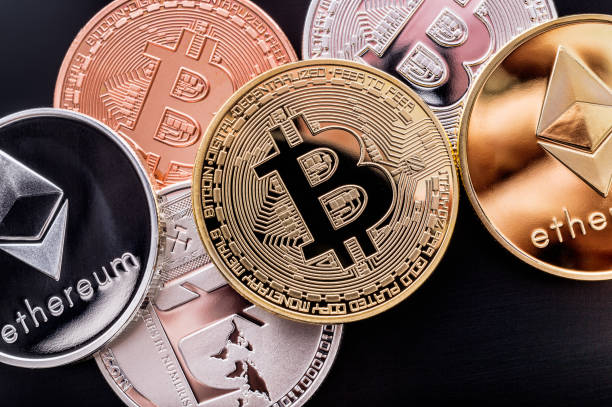
\includegraphics[scale=1.6]{crypto}
	\begin{itemize}
		\item Share what you know, have heard, have seen, etc.! \pause
		\item \textcolor{blue}{\href{https://jamboard.google.com/d/11aMUTrsNXKniKVkajcfThbODdwsedcUUsrVuGIbXTAo/edit?usp=sharing}{Group Jamboarding Session!}}
	\end{itemize}
\end{frame}
%%%%%%%%%%%% Slide %%%%%%%%%%%%%%%%%%%%%%%%%%%%%%%%%%%%%%%%%%%%%%%%%%%
\begin{frame}
  \frametitle{Bitcoin vs. bitcoin vs. Blockchain}
  
	\begin{block}{\textbf{\textcolor{brown}{Bitcoin:}}}
	Concepts and technologies that form the basis of a digital money ecosystem (cryptocurrency).
	\end{block}

    \pause
    
	\begin{block}{\textbf{\textcolor{brown}{bitcoin:}}}
	Unit of digital currency.
	\end{block}
	
	\pause
	
	\begin{block}{\textbf{\textcolor{brown}{Blockchain}}}

	A public transaction ledger (a data structure).

	\end{block}
\end{frame}

%%%%%%%%%%%% Slide %%%%%%%%%%%%%%%%%%%%%%%%%%%%%%%%%%%%%%%%%%%%%%%%%%%
\begin{frame}
  \frametitle{Bitcoin}
	\begin{itemize}
		\item 2008: The Bitcoin white paper
		
	\begin{tabular}{ll}
	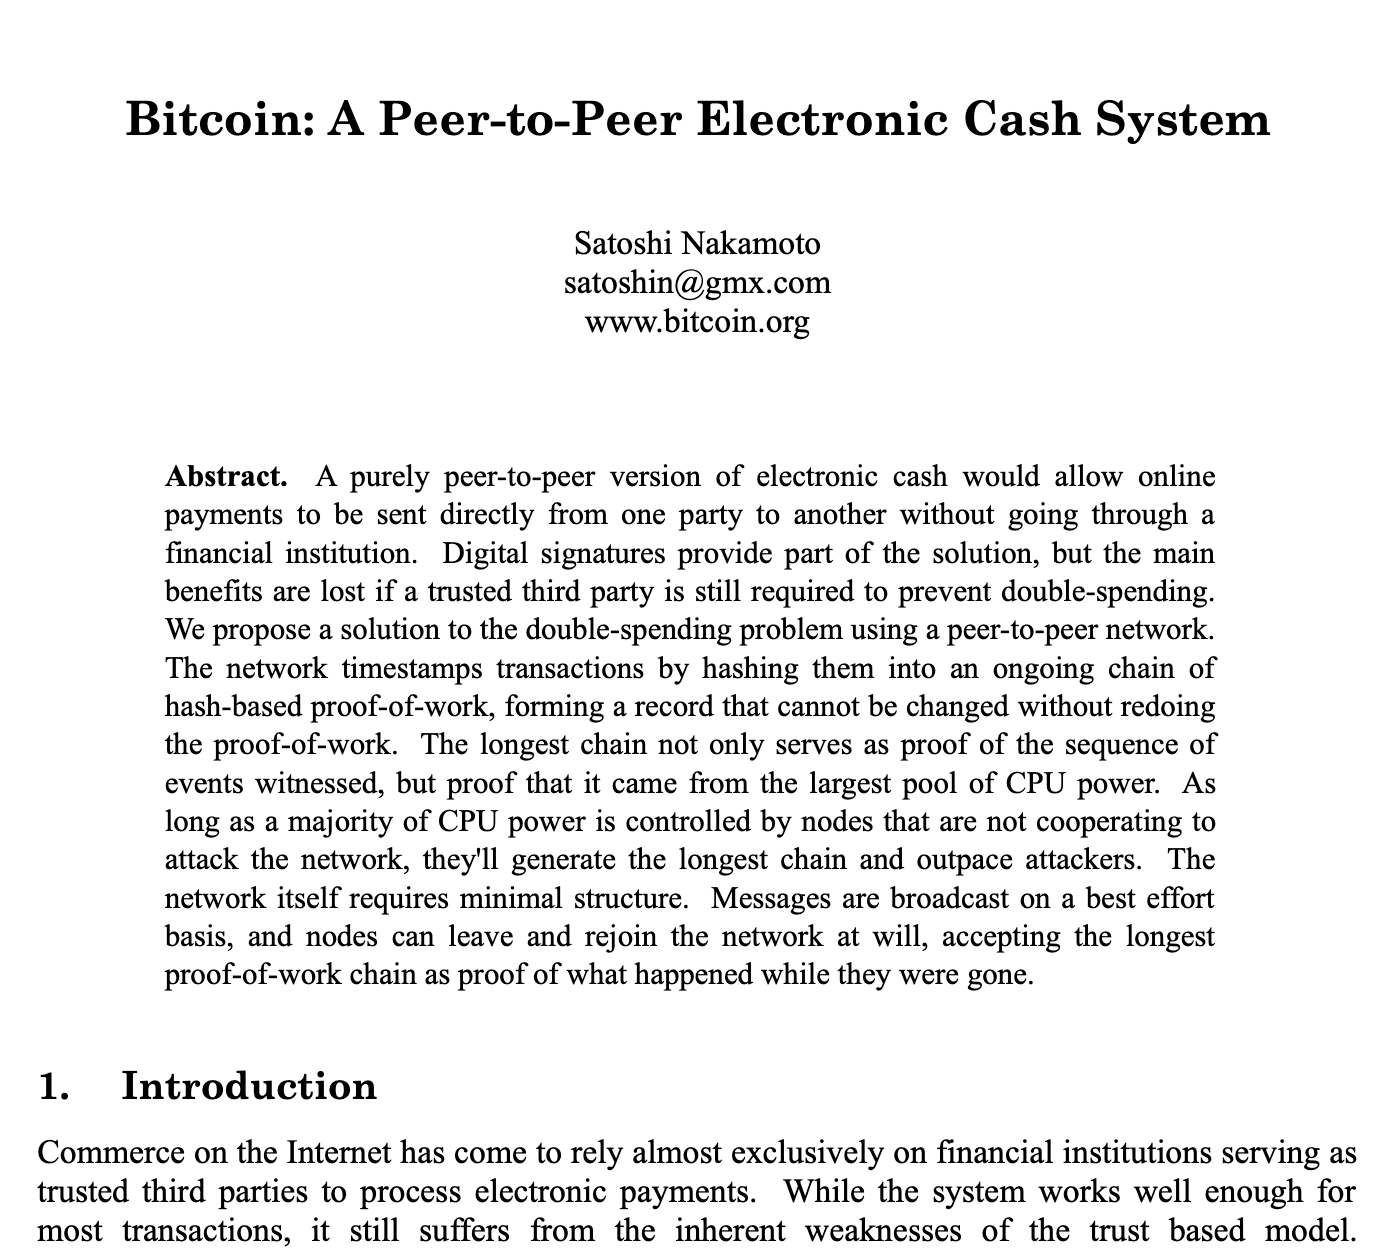
\includegraphics[scale=0.25]{Bitcoin_paper} &
	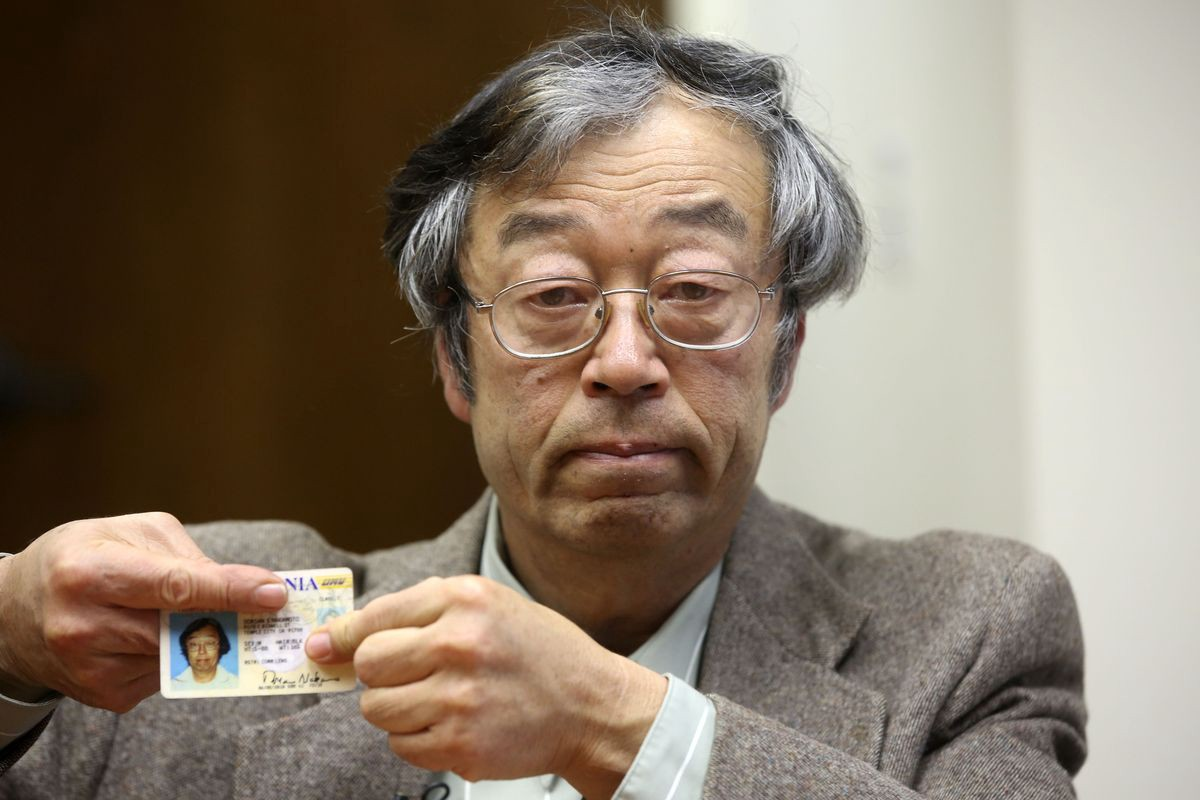
\includegraphics[scale=0.12]{satoshi} \\ & \hspace{0.5in} Not this guy!
	\end{tabular}
	\pause
		\item 2009: Reference implementation
	\end{itemize}
\end{frame}

%%%%%%%%%%%% Slide %%%%%%%%%%%%%%%%%%%%%%%%%%%%%%%%%%%%%%%%%%%%%%%%%%%
\begin{frame}
  \frametitle{Cryptocurrency Prices by Market Cap}
	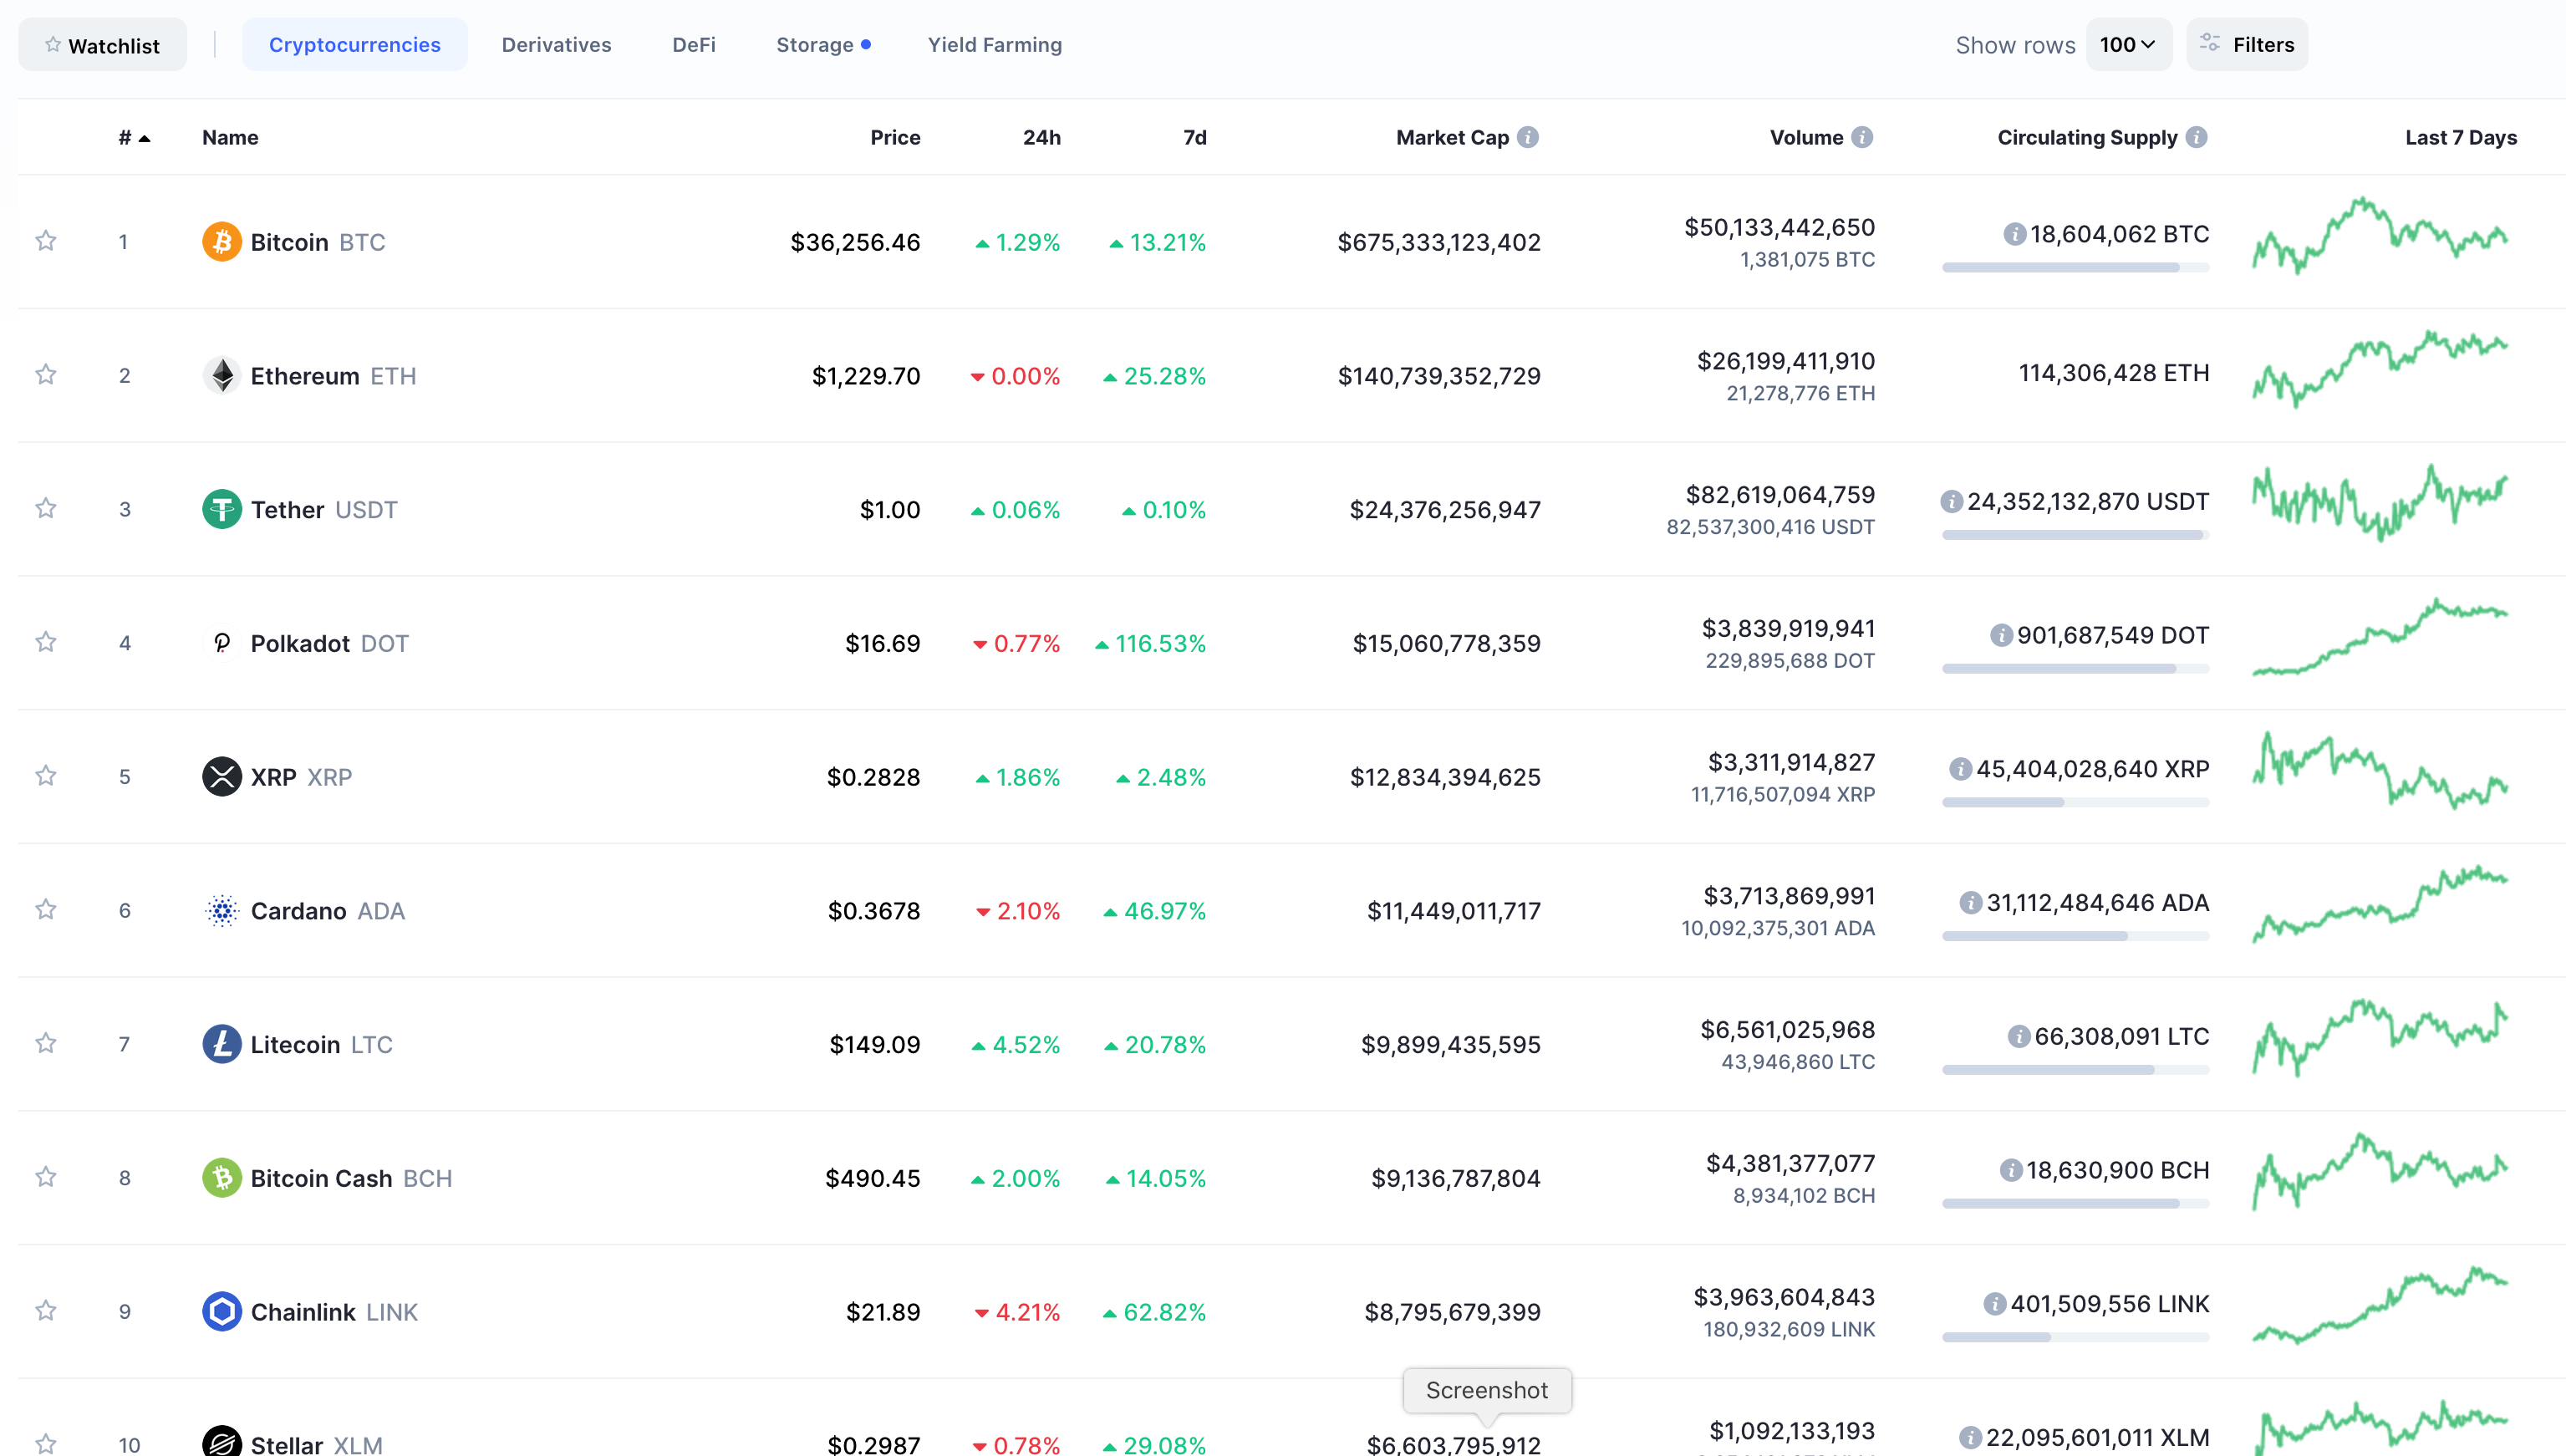
\includegraphics[scale=0.2]{market}
	{\tiny{\url{https://coinmarketcap.com/} as of January 18, 2021.}}
	
	Rewards and Fees: \url{https://www.blockchain.com/stats}
\end{frame}

%%%%%%%%%%%% Slide %%%%%%%%%%%%%%%%%%%%%%%%%%%%%%%%%%%%%%%%%%%%%%%%%%%
\begin{frame}
  \frametitle{Trust?}
  \centering
	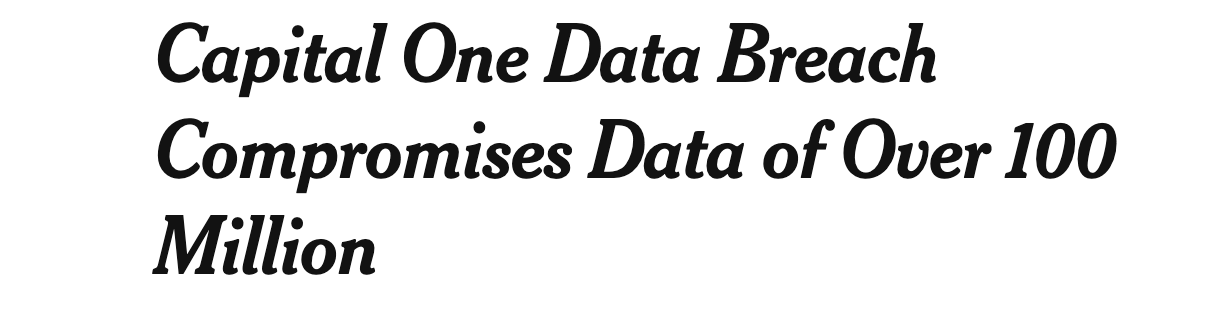
\includegraphics[scale=0.25]{capitalone}
	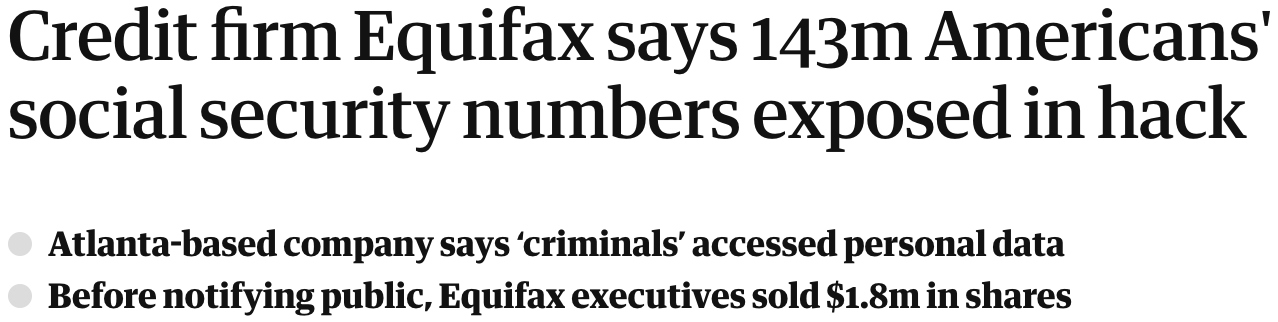
\includegraphics[scale=0.25]{equifax} 
	
\includegraphics[scale=0.25]{bank}
	\pause
	
	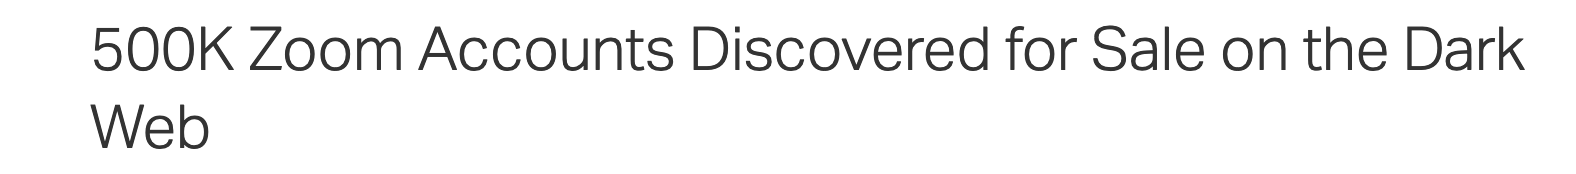
\includegraphics[scale=0.2]{zoom}
	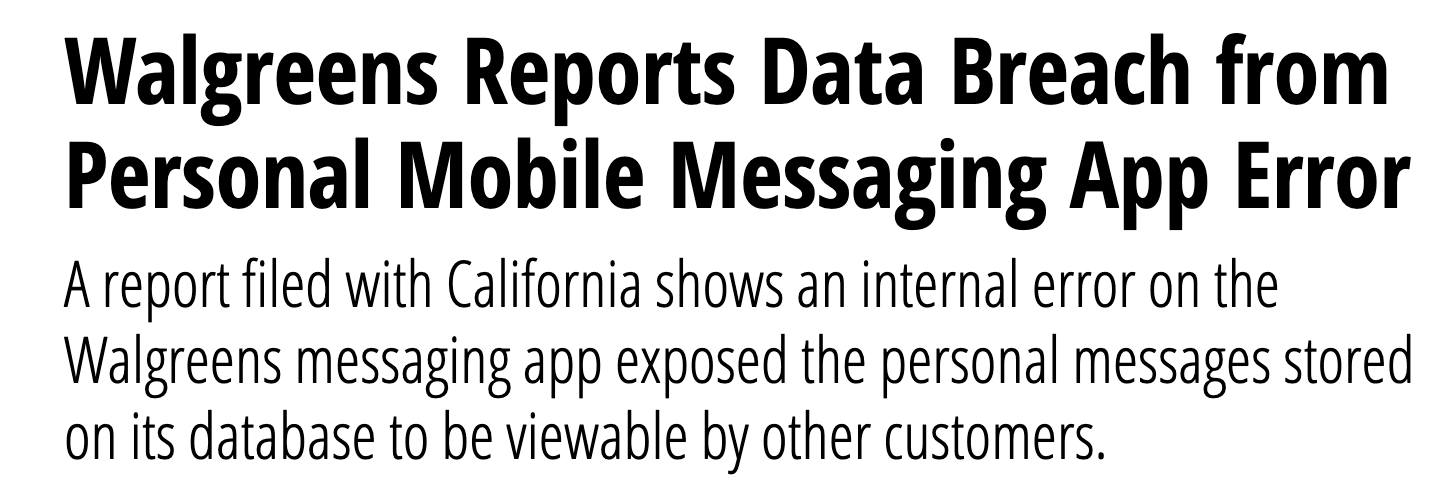
\includegraphics[scale=0.2]{walgreens}
	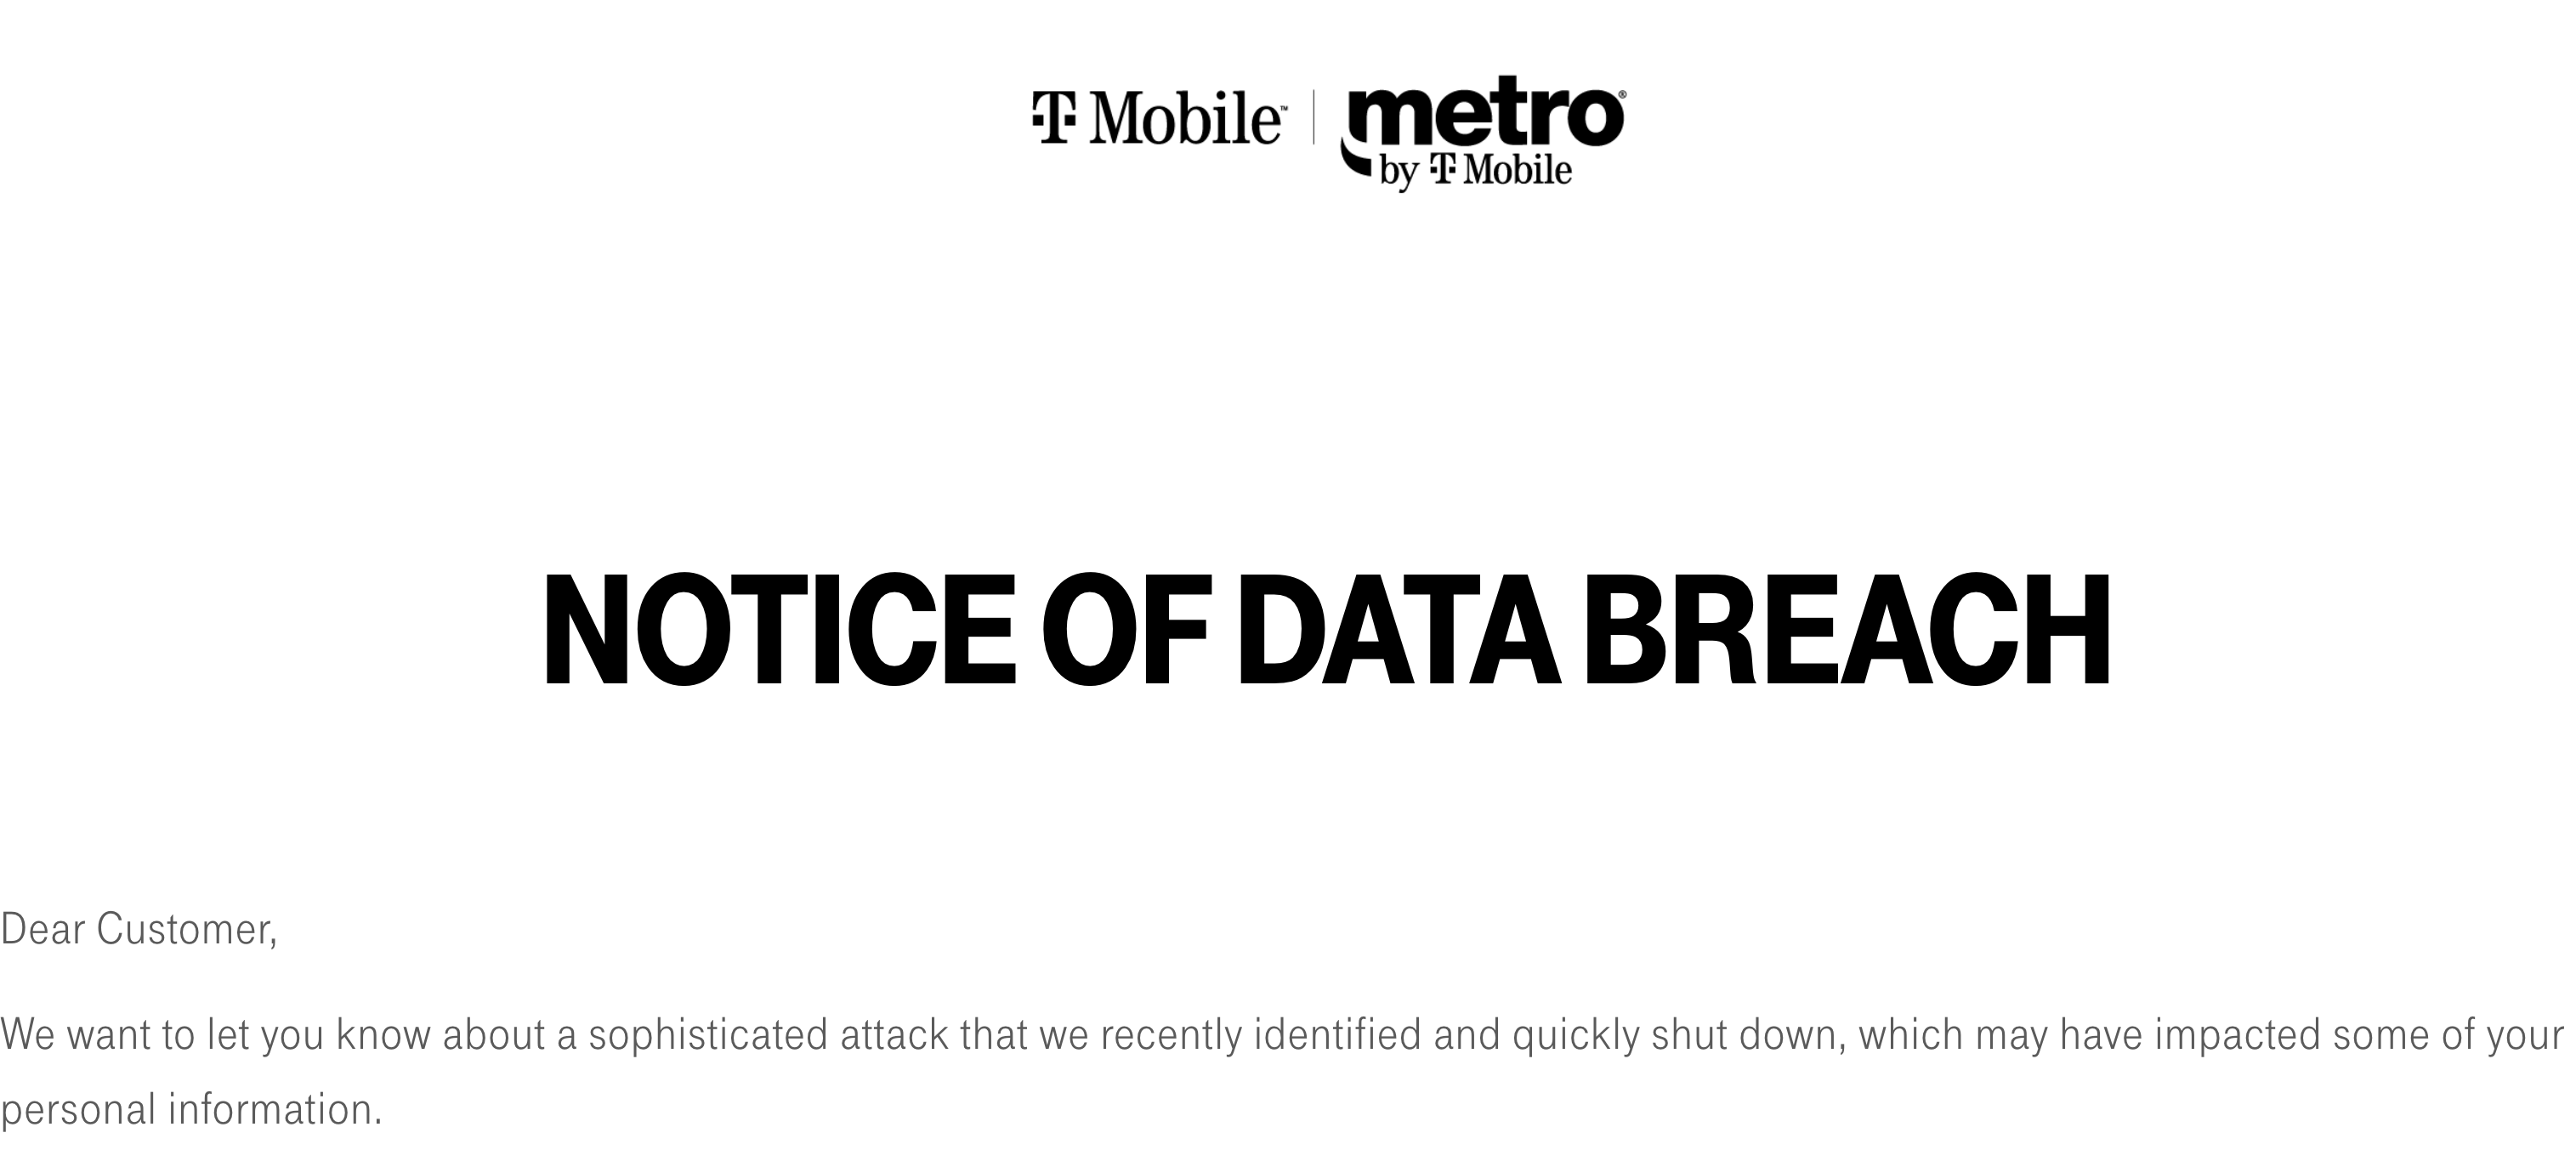
\includegraphics[scale=0.15]{metro}
\end{frame}
%%%%%%%%%%%% Slide %%%%%%%%%%%%%%%%%%%%%%%%%%%%%%%%%%%%%%%%%%%%%%%%%%%
\begin{frame}
  \frametitle{Decentralization}
  \centering 
  	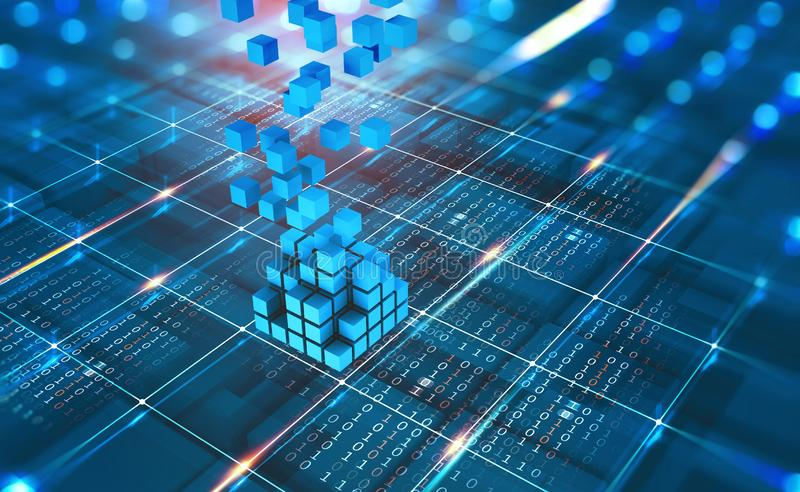
\includegraphics[scale=1]{blockchain}
  	
  \begin{itemize}
 	\item  Here comes Blockchain! \\
  
 	\item  First, let's see what questions we need to think about answering. \\
	Take \href{https://forms.gle/BkPfQSLQhpNSNfkf6}{\textcolor{blue}{ the pre-survey}}
 \end{itemize}
\end{frame}
%%%%%%%%%%%% Slide %%%%%%%%%%%%%%%%%%%%%%%%%%%%%%%%%%%%%%%%%%%%%%%%%%%
\begin{frame}
  \frametitle{Blockchain}
	\begin{itemize}
		\item \textcolor{brown}{Decentralized control}: consensus of the community.
		\item \textcolor{brown}{Tamper-evidence:} can immediately detect data tampering.
		\item \textcolor{brown}{Nakamoto consensus:} have to provably spend resources when updating the blockchain.
	\end{itemize}
\end{frame}
%%%%%%%%%%%% Slide %%%%%%%%%%%%%%%%%%%%%%%%%%%%%%%%%%%%%%%%%%%%%%%%%%%
\begin{frame}
  \frametitle{Centralization vs. Decentralization}
	\begin{block}{\textbf{\textcolor{brown}{Centralization:}}}
	\begin{itemize}
		\item Authority by a single party.
		\item Data stored by a single party.
	\end{itemize}
	\end{block}

    \pause
    
	\begin{block}{\textbf{\textcolor{brown}{Decentralization:}}}
	\begin{itemize}
		\item Authority according to a public protocol.
		\item Data stored by the participants.
	\end{itemize}
	\end{block}
	
	\pause
	
	\centering
	\begin{tabular}{ll}
		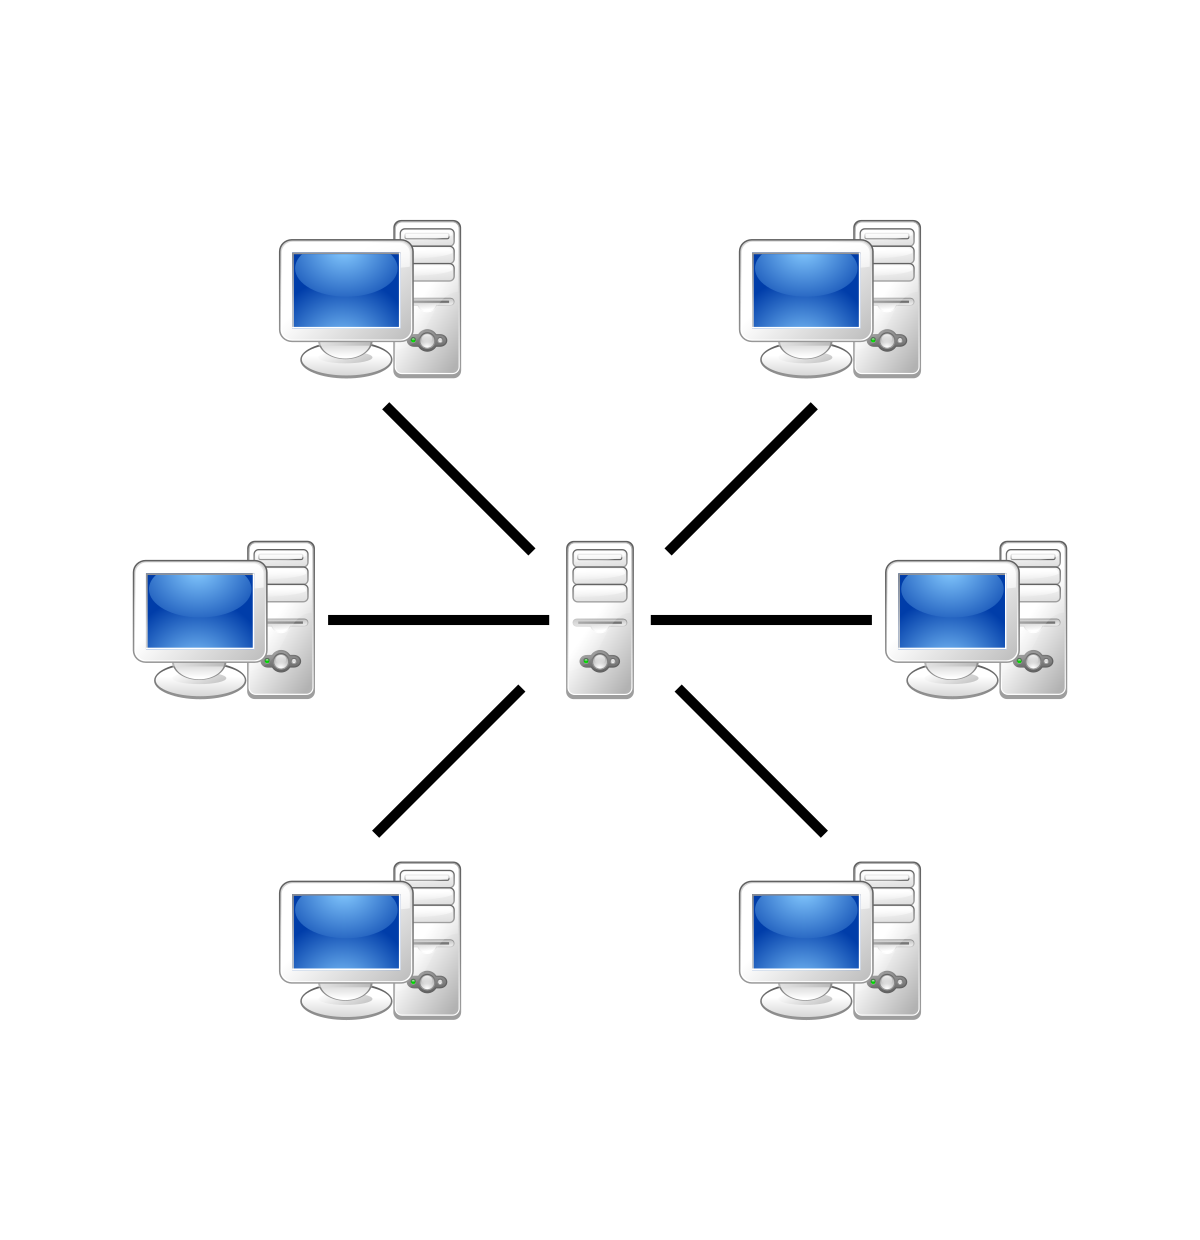
\includegraphics[scale=0.05]{centralized} \hspace{0.5in} &
		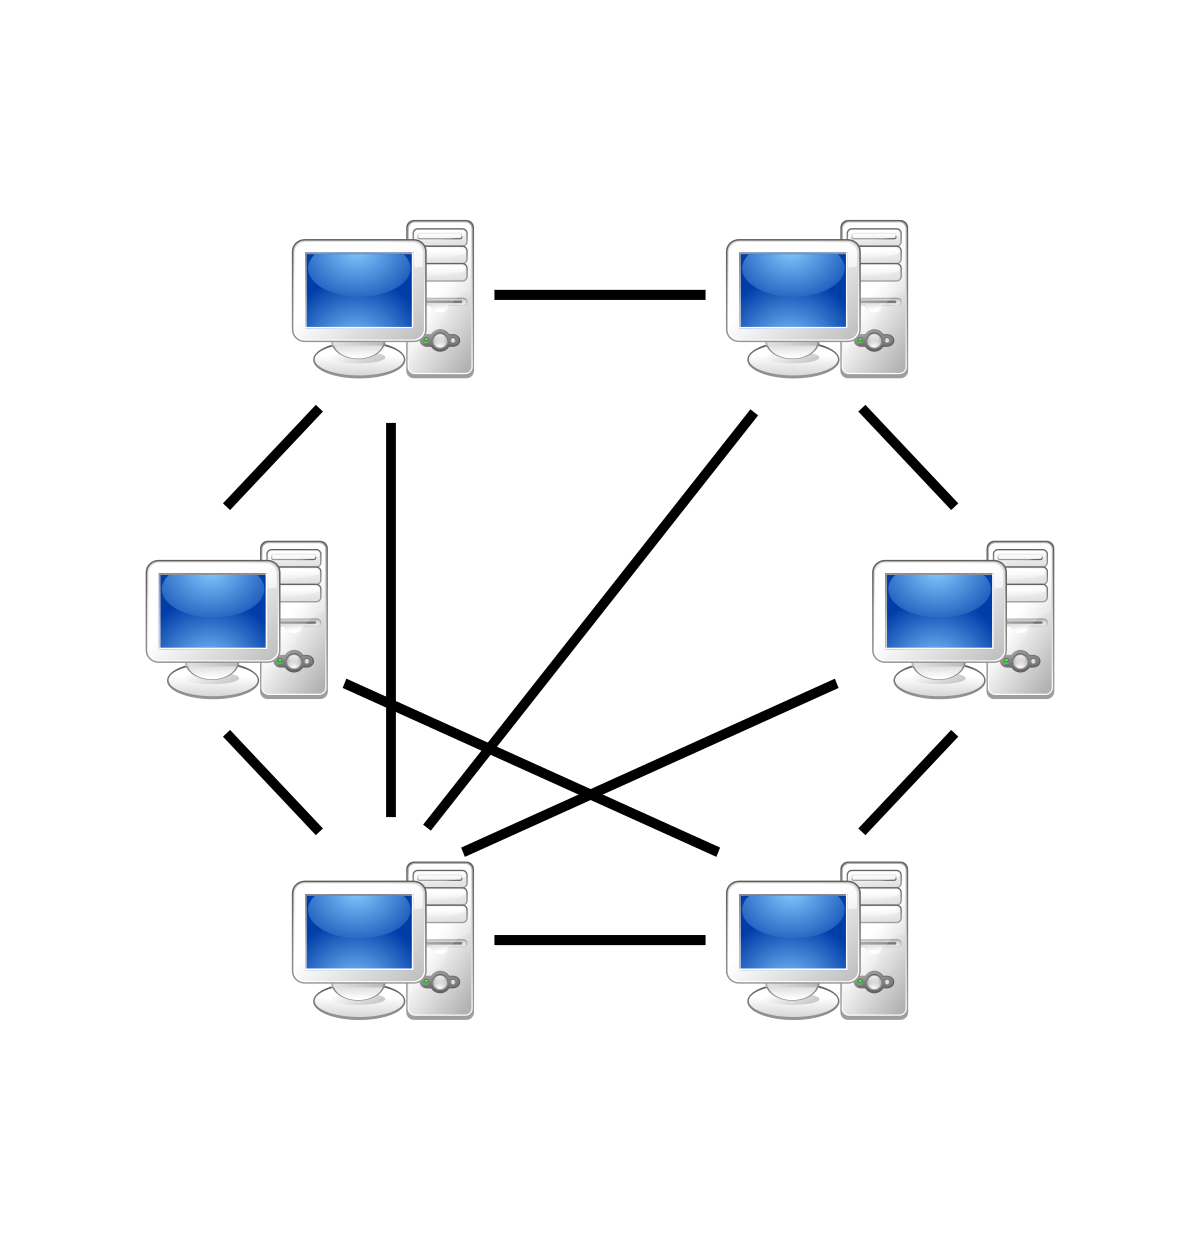
\includegraphics[scale=0.05]{decentralized} \\
		client-server & peer-to-peer
	\end{tabular}
\end{frame}
%%%%%%%%%%%% Slide %%%%%%%%%%%%%%%%%%%%%%%%%%%%%%%%%%%%%%%%%%%%%%%%%%%
\begin{frame}
  \frametitle{Cryptocurrency Components}
	\begin{itemize}
		\item \textcolor{brown}{Identity}:  an account (\textcolor{brown}{node}) in the system.
		\item \textcolor{brown}{Transactions:} sending and receiving  units of cryptocurrency.
		\item \textcolor{brown}{Distributed Ledger:} a public record of transaction history (blockchain).
		\item \textcolor{brown}{Trustless Consensus:} agreement on changes to the ledger.
	\end{itemize}
\end{frame}
%%%%%%%%%%%% Slide %%%%%%%%%%%%%%%%%%%%%%%%%%%%%%%%%%%%%%%%%%%%%%%%%%%
\begin{frame}
  \frametitle{Identity: Private and Public Keys}
	\begin{itemize}
		\item \textcolor{brown}{Public Key}:  represents an identity, used for ``receiving''.
		\item \textcolor{brown}{Private Key:}  ``unlocks'' public key and the money, used for ``redeeming''. \\
	\pause
	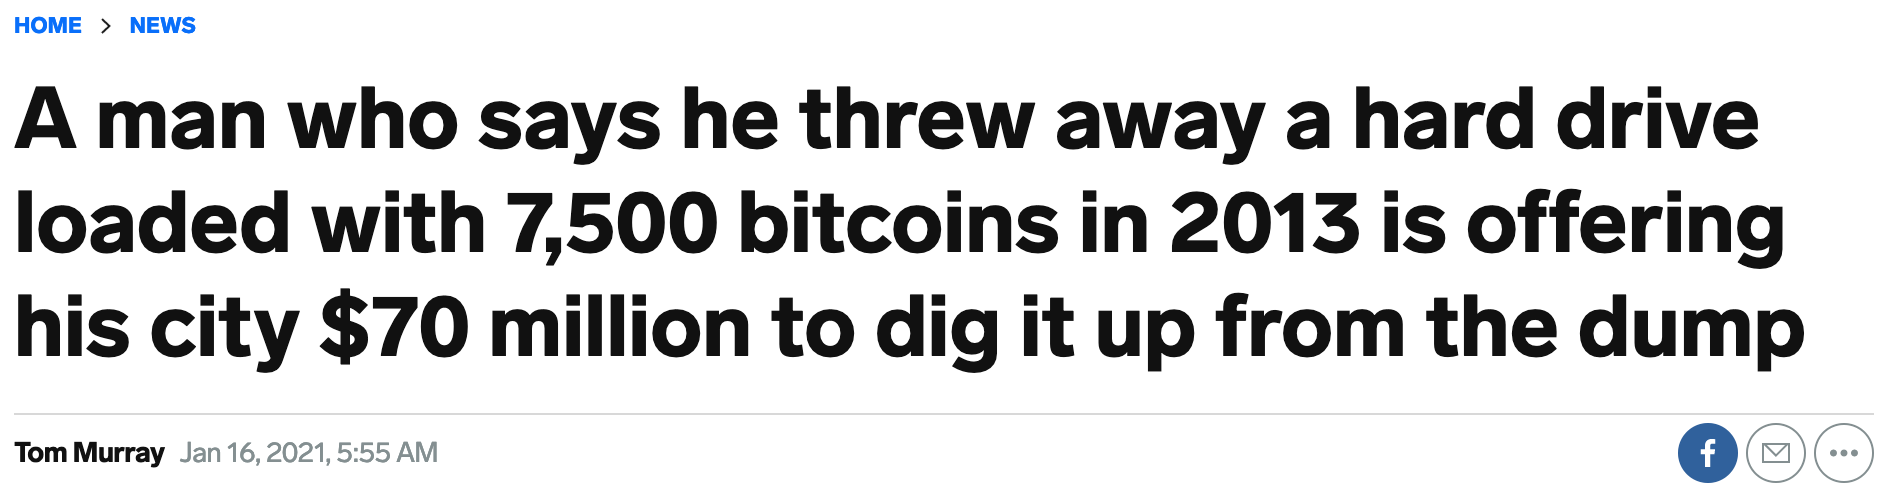
\includegraphics[scale=0.2]{trash}
	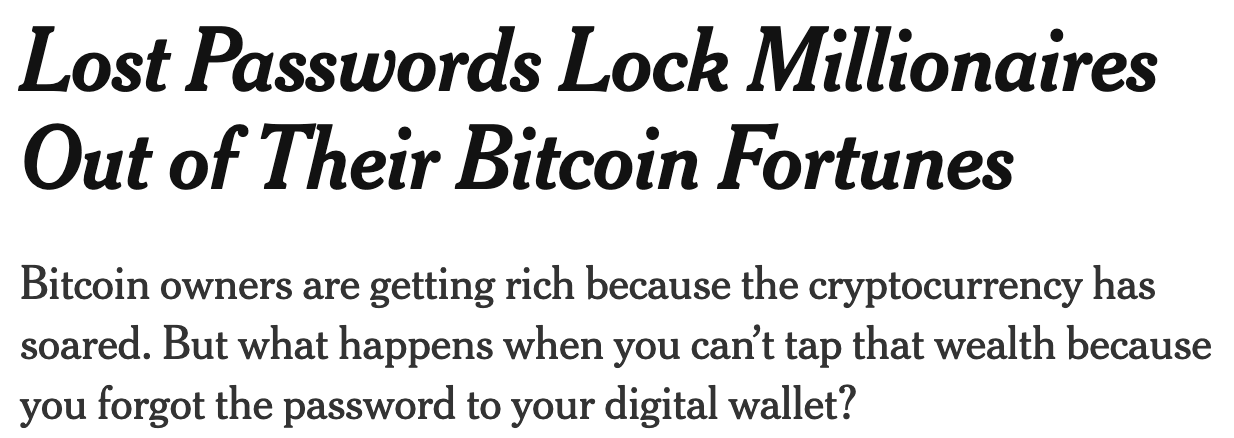
\includegraphics[scale=0.2]{password}
	\textcolor{red}{Don't be this guy!}
	\pause
		\item  \textcolor{brown}{A bitcoin address:} representation of the recipient's public key, generated using cryptographic hash function. \\
		
			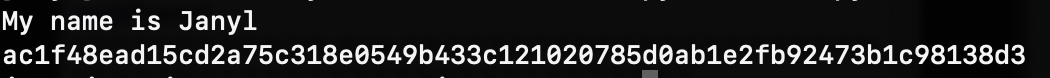
\includegraphics[scale=0.5]{hash}
	\end{itemize}
\end{frame}
%%%%%%%%%%%% Slide %%%%%%%%%%%%%%%%%%%%%%%%%%%%%%%%%%%%%%%%%%%%%%%%%%%
\begin{frame}
  \frametitle{Transactions}
	\begin{itemize}
		\item Transactions are processed during a process called \textcolor{brown}{mining}.
		\item Miners use computational power to verify and record transactions are rewarded with new bitcoin.
	\end{itemize}
	\centering
	\begin{tabular}{ll}
	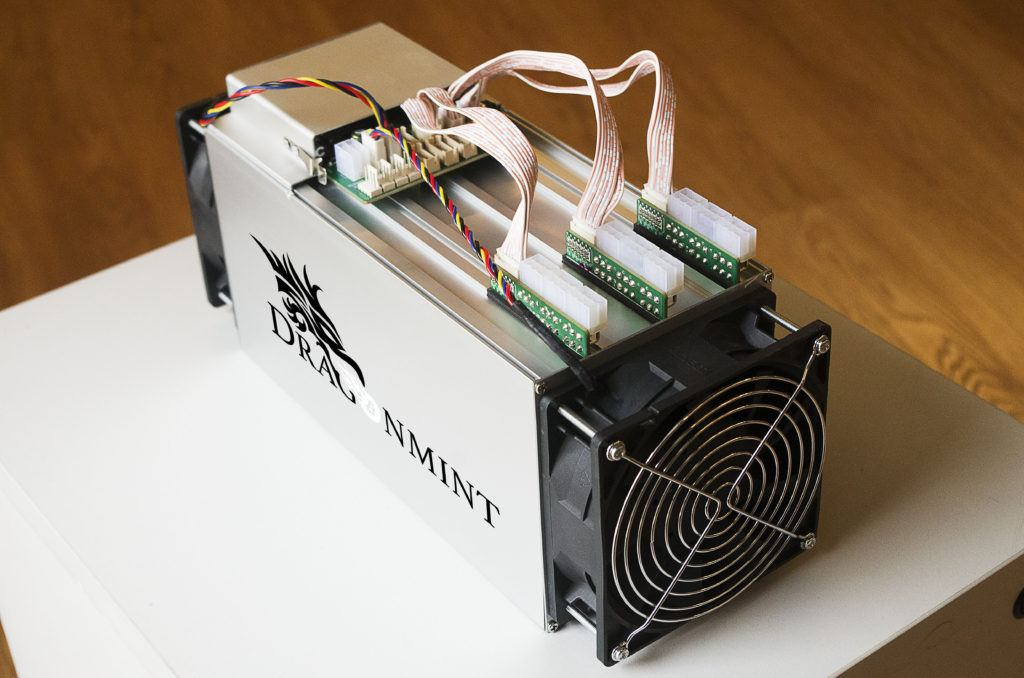
\includegraphics[scale=0.15]{dragonmint.jpg} &
	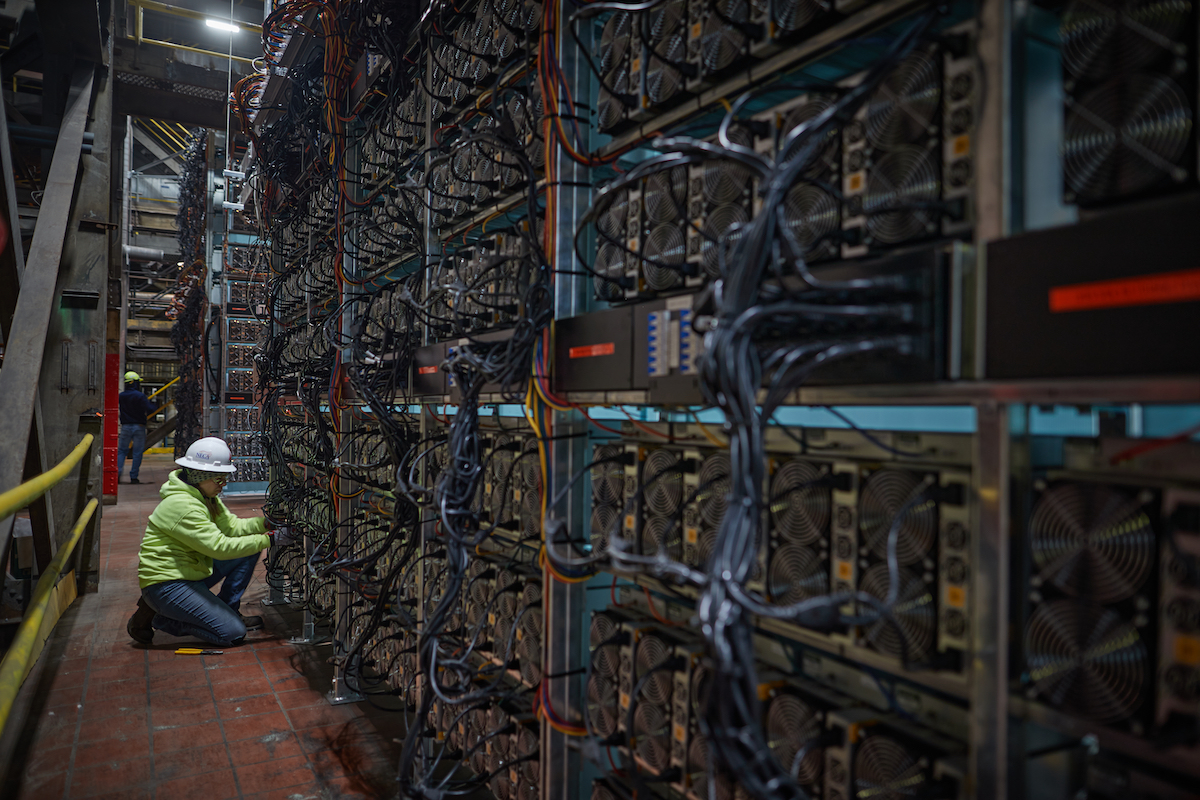
\includegraphics[scale=0.13]{mining.jpg} 
	\end{tabular}
\end{frame}
%%%%%%%%%%%% Slide %%%%%%%%%%%%%%%%%%%%%%%%%%%%%%%%%%%%%%%%%%%%%%%%%%%
\begin{frame}
  \frametitle{Distributed Ledger: Record Keeping using Blockchain}
	\begin{itemize}
		\item Data is stored by everyone.
		\item Updates are broadcasted to everyone.
		\item Transactions are bundled into \textcolor{brown}{blocks} with links to enforce ordering.
		\item Miner creates a block by verifying transactions and solving a hashing problem.
	\end{itemize}

\end{frame}
%%%%%%%%%%%% Slide %%%%%%%%%%%%%%%%%%%%%%%%%%%%%%%%%%%%%%%%%%%%%%%%%%%
\begin{frame}
  \frametitle{Consensus}
	\begin{itemize}
		\item Process by which participants come to agreement (e.g., making changes to a ledger of transactions).
		\item Transactions are approved by \textcolor{brown}{Proof-of-Work}.
	\end{itemize}
	 $ $ \\ $ $
	\pause
	{\huge{More details on the process involved in blockchain next class!}}
\end{frame}
%%%%%%%%%%%% Slide %%%%%%%%%%%%%%%%%%%%%%%%%%%%%%%%%%%%%%%%%%%%%%%%%%%
\end{document}
